\chapter{Entrada d'Àudio Digital}
\section{Font d'àudio digital}
\par Per transmetre a l'entrada de l'amplificador un senyal d'àudio en protocol I2S, s'ha emprat una targeta ESP32-WROOM-32 juntament amb un lector de targetes microSD controlat per SPI. 
 \par El tamany de la memòria RAM de l'ESP32 és de 520 kBytes i per reproduir arxius d'àudio com el d'una cançó es necessiten de l'ordre de MBytes; és per això que per emmagatzemar arxius de major tamany, s'ha utilitzat el mòdul adaptador de targetes microSD, per poder fer la lectura del contingut mitjançant el protocol SPI.
 \par Per implementar la font d'àudio, s'han emprat els següents dispositius i components:
 \begin{itemize}
     \item \textbf{Targeta ESP32-WROOM-32:} Aquesta targeta inclou el MCU encarregat de llegir la targeta microSD i transmetre la informació pel bus I2S.
     \begin{figure}[H]
         \centering
         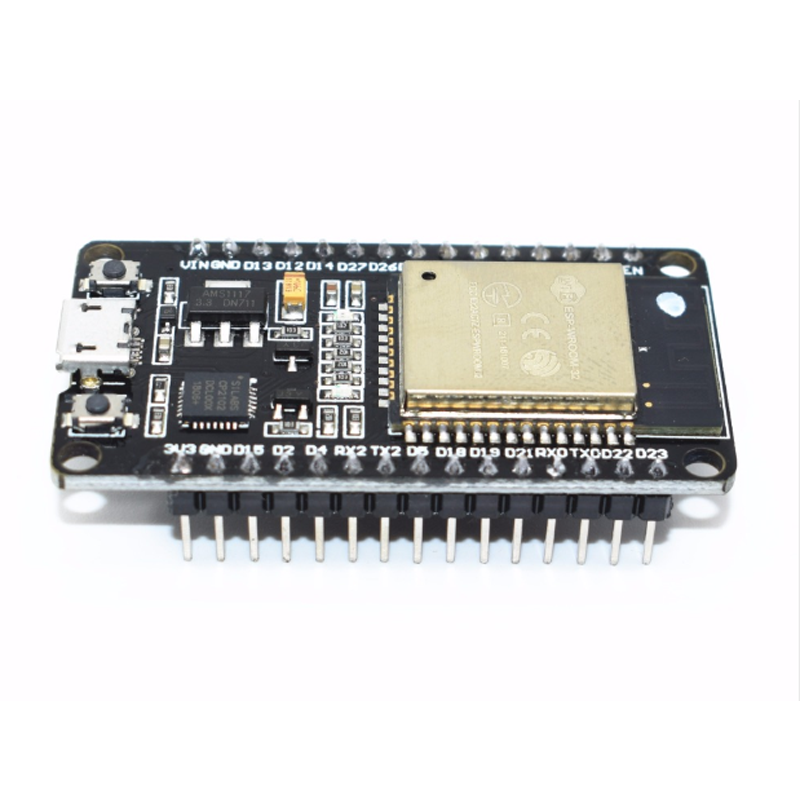
\includegraphics[width=0.25\linewidth]{Images/wroom-32-v2.jpg}
         \caption{Targeta MCU del ESP32-WROOM-V2.}
         \label{ESP32_fig}
     \end{figure}
     \item \textbf{Mòdul adaptador de la targeta microSD:} Aquest mòdul està pensat per poder utilitzar-lo amb tota la gamma de productes d'Arduino, per això a més del suport per a la targeta microSD, inclou un LDO de 3V3 i un Level-shifter que en cas d'utilitzar una placa Arduino amb lògica de 5 V, no faci malbé la targeta.
     \begin{figure}[H]
         \centering
         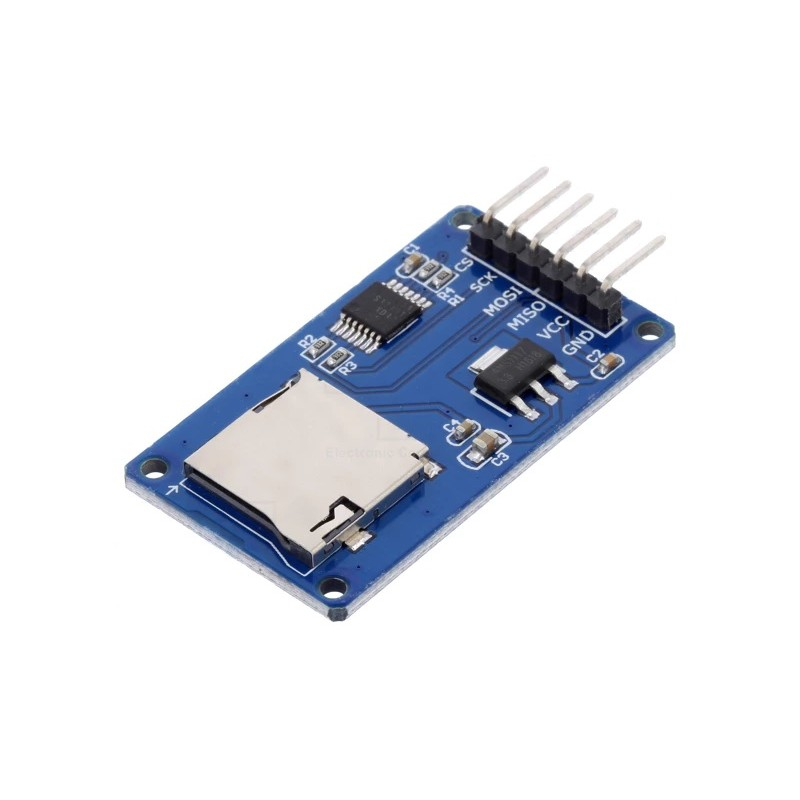
\includegraphics[width=0.25\linewidth]{Images/microsd_arduino.jpg}
         \caption{Adaptador de targeta microSD a SPI.}
         \label{microSD_adapter_fig}
     \end{figure}
     \item \textbf{Mòdul d'alimentació 5 V:} Per poder comunicar-se amb la targeta microSD, com s'ha mencionat en l'anterior ítem, el mòdul adaptador de la targeta microSD ha d'estar alimentat a 5 V. 
     \begin{figure}[H]
         \centering
         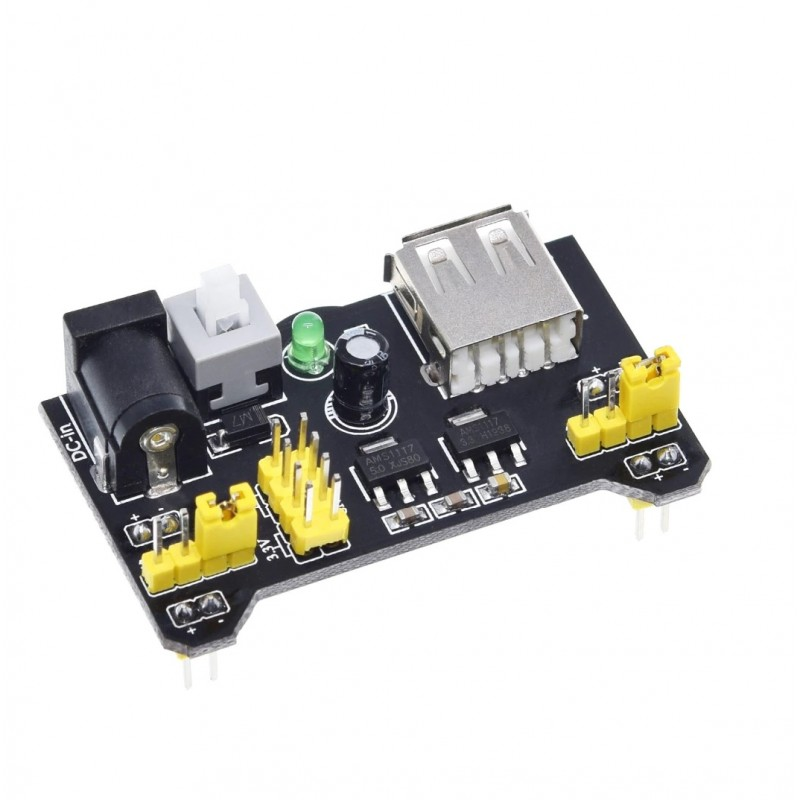
\includegraphics[width=0.25\linewidth]{Images/modulo-arduino-alimentacion.jpg}
         \caption{Mòdul alimentació 5V i 3,3V.}
         \label{modul_supply_fig}
     \end{figure}
     \item \textbf{Targeta microSD:} La targeta microSD on es guarden els arxius d'àudio en format .wav, és el model microSD Ultra de 8 GBytes.
    \begin{figure}[H]
        \centering
        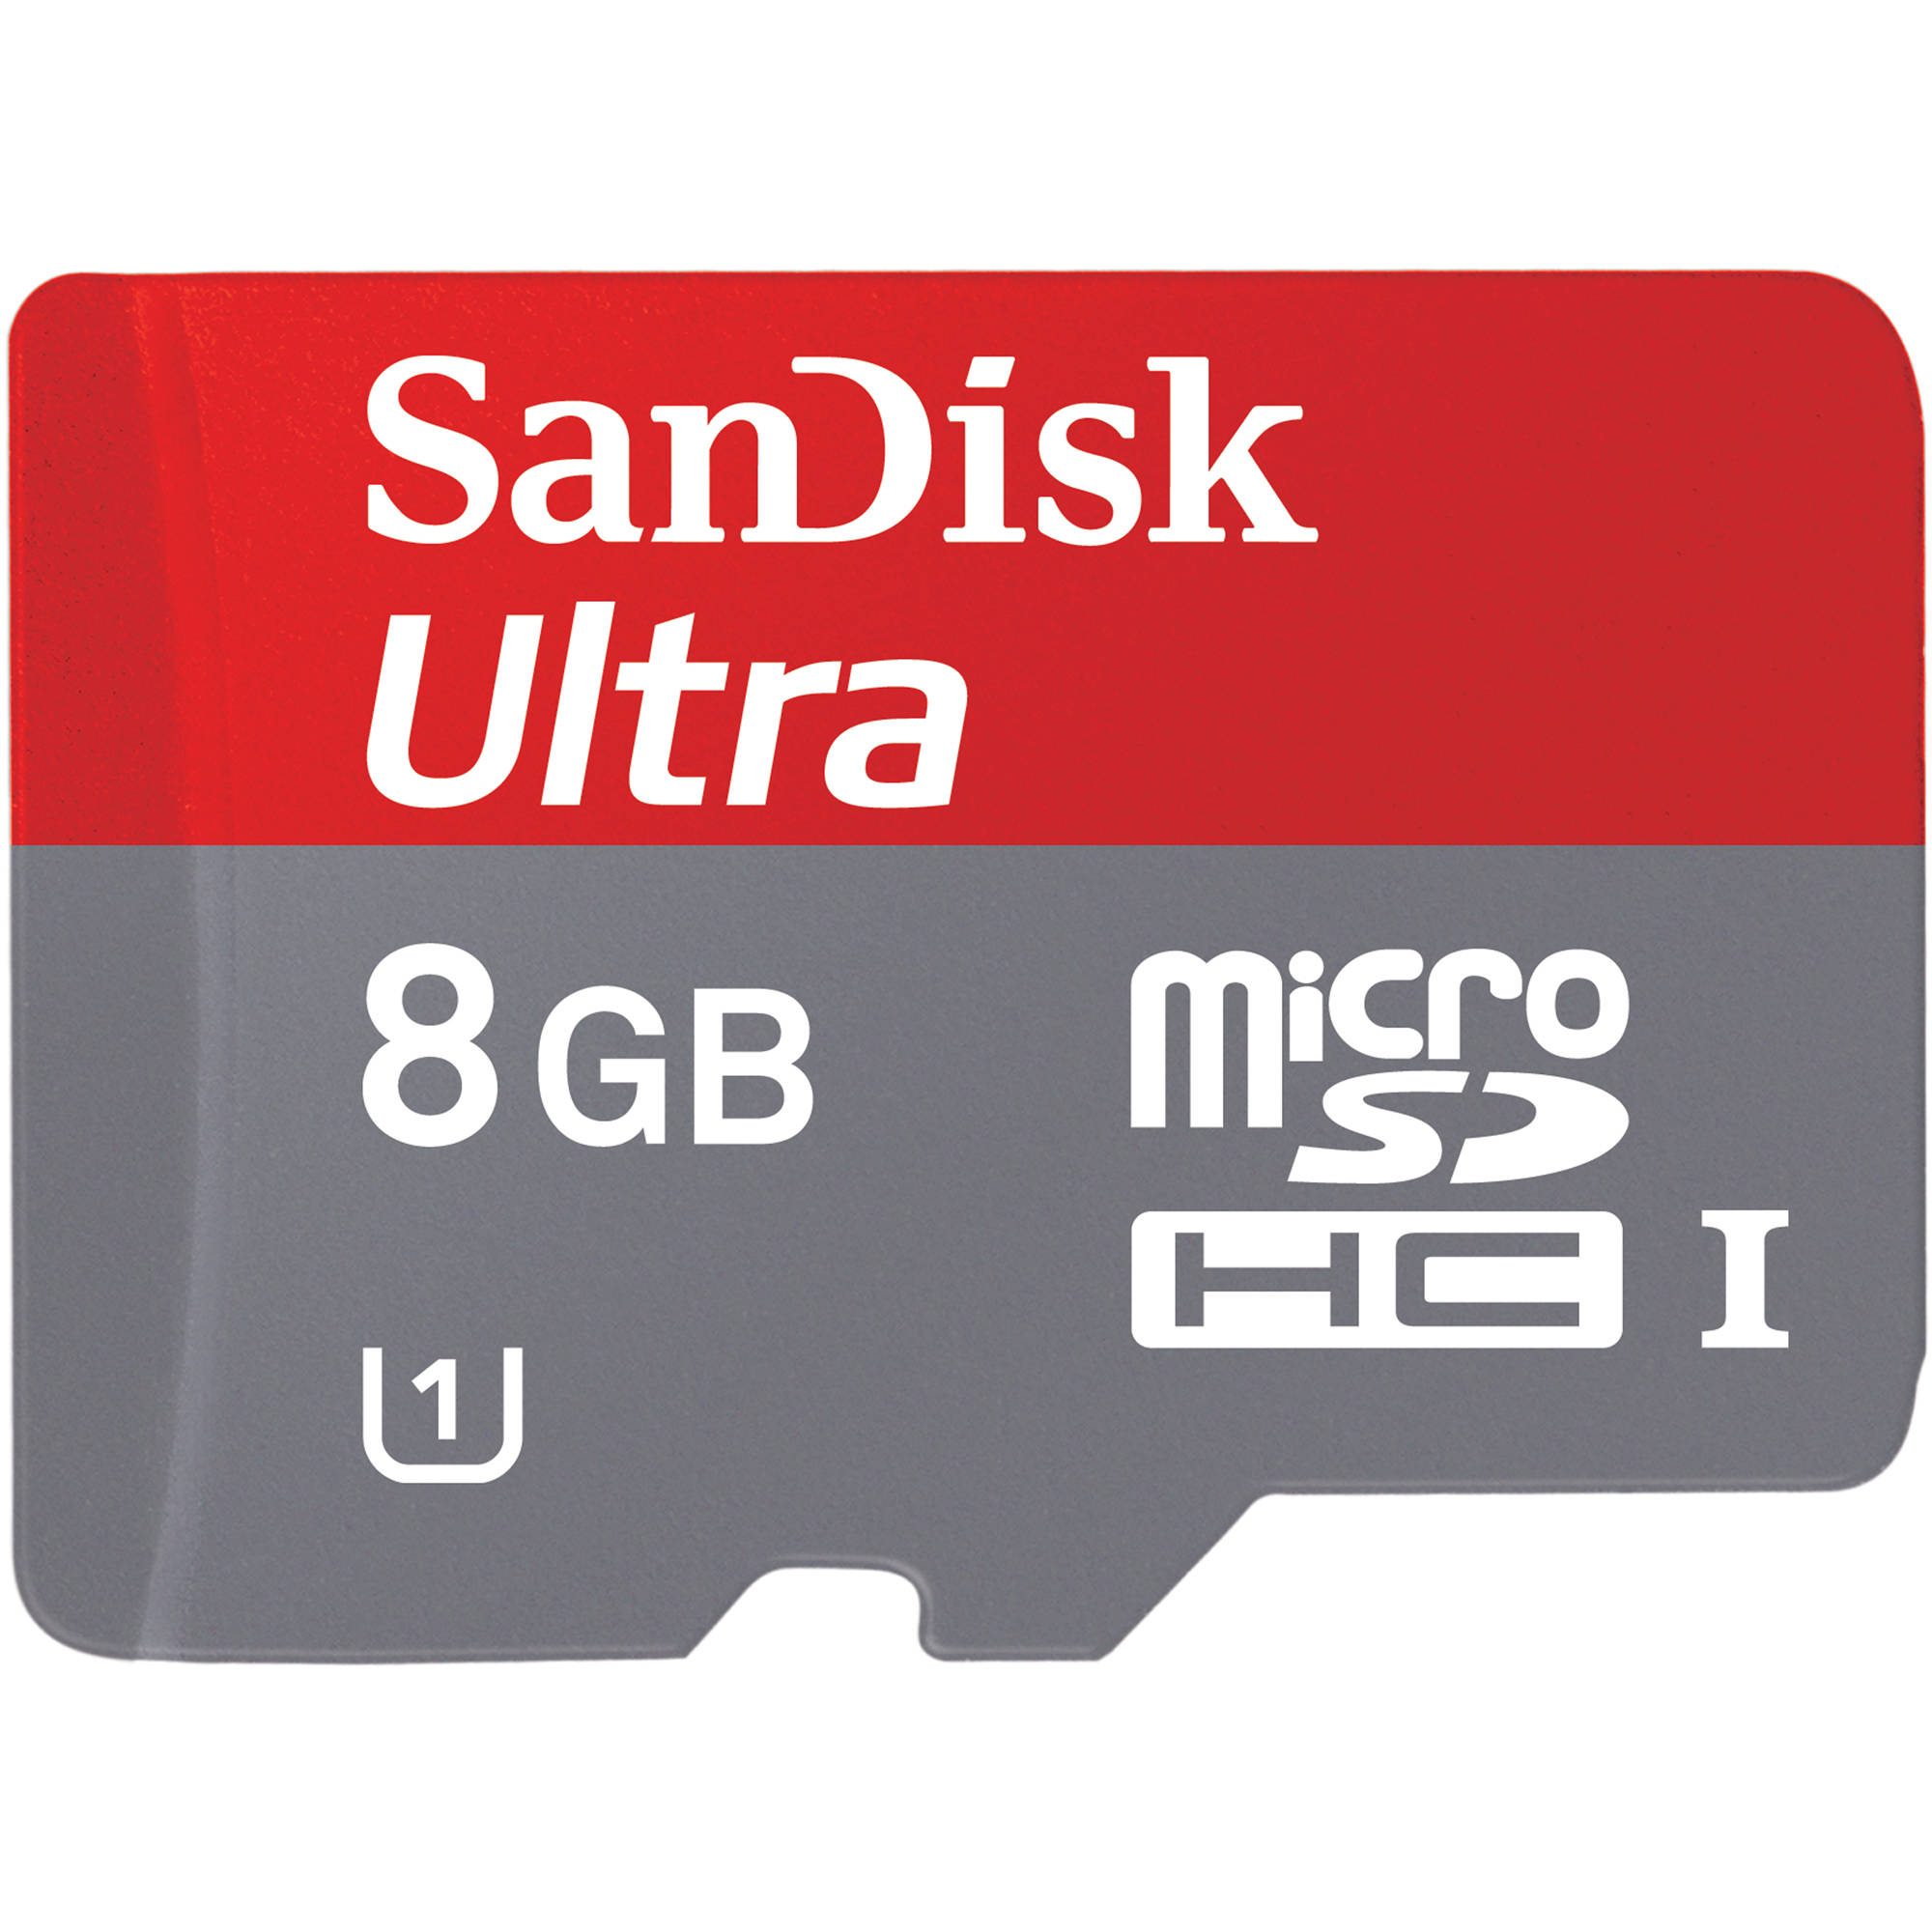
\includegraphics[width=0.15\linewidth]{Images/microsd_8gb.jpg}
        \caption{Targeta microSD amb 8 Gb de memòria.}
        \label{microSD_fig}
    \end{figure}
 \end{itemize}

\subsection{Llibreria SD.h}
\par La llibreria SD.h permet fer lectures de targetes SD i escriure-hi, tot utilitzant un seguit de funcions que a continuació es mencionen.
\par Per inicialitzar la targeta SD, cal cridar la funció \textit{begin()} i, si escau, especificar el pin de CS. La funció \textit{begin()} retorna una variable de tipus bool per poder determinar si s'ha inicialitzat correctament la comunicació amb la targeta SD.
\begin{figure}[H]
    \centering
    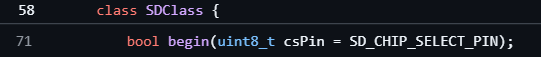
\includegraphics[width=0.5\linewidth]{Images/SD-begin_method.png}
    \caption{Mètode begin() de la classe SDclass. (font arduino o repo github)}
    \label{SD_begin_method_fig}
\end{figure}
\par Un cop inicialitzada correctament la targeta SD i el protocol SPI per la comunicació entre SD i ESP32, es poden obrir els fitxers emmagatzemats dins la SD. Amb la funció \textit{open(filepath)}, s'obre l'arxiu especificat al directori i en genera un objecte de la classe file o, en cas de no existir cap fitxer sota l'adreça de l'argument, retorna un false en booleà. D'aquesta forma, l'objecte generat a partir del fitxer permet fer ús dels mètodes de la classe file com llegir el seu contingut (\textit{read(*direcció memòria, longitud en bytes)}) i accedir a una direcció concreta dins la memòria (\textit{seek(*direcció memòria)}), entre d'altres.\cite{SDarduino}

\subsection{Llibreria I2S.h}
\par La targeta ESP32-WROOM-32 conté dos perifèrics I2S que es poden configurar per transmetre la informació en mode master o slave i actuar com un transmissor o receptor d'informació.
\par La targeta ESP32 s'ha configurat en mode master transmissora degut a les necessitats del sistema implementat.
\par Per configurar el mode de treball del canal I2S entre altres propietats, cal declarar l'struct \textit{i2s{\_}config{\_}t}. A la figura \ref{i2s_config_fig}, es pot observar la declaració de la variable constant de tipus estàtic \textit{i2s{\_}config} per configurar els paràmetres del protocol I2S. El primer atribut és el mode d'operació del port declarat, que és una variable de tipus enum. El mode predeterminat és de master transmissor \cite{I2SESP32code}. El segon atribut és la freqüència de sampleig de la informació transmesa pel bus. El tercer atribut és una nova variable enum, \textit{i2s{\_}bits{\_}per{\_}sample{\_}t}, que especifica el tamany de les mostres. L'atribut \textit{channel{\_}format} especifica el format de la trama del bus I2S. Com es comentarà més endavant, el format emprat és l'estàndard de Phillips, degut a que el transceiver dissenyat a la FPGA s'ha plantejat amb aquest mode d'operació. Per últim a destacar de l'struct \textit{i2s{\_}config}, l'atribut \textit{communication{\_}format} és una variable enum que especifica el format de comunicació de la mostra pel port SD. Els atributs que resten son per declarar la variable d'interrupció i els tamanys dels buffers emprats per la transmissió de les mostres, entre d'altres; es deixen en el mode predeterminat.

\begin{figure}[H]
    \centering
    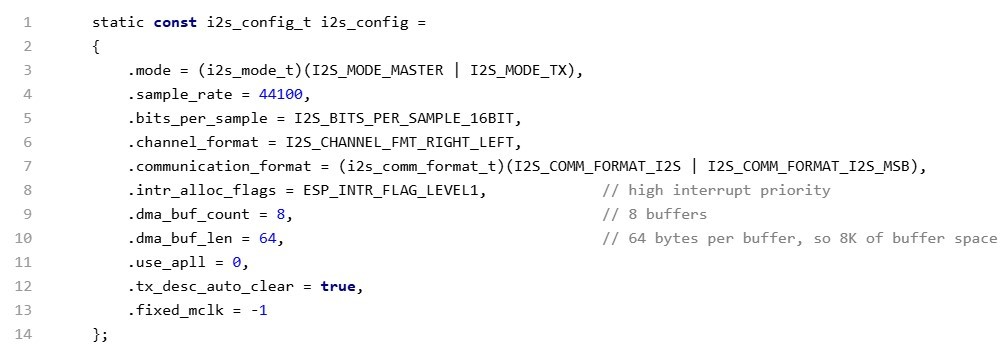
\includegraphics[width=0.7\linewidth]{Images/codi_i2sconfig.jpeg}
    \caption{Extracte del codi emprat per programar la targeta ESP32, on es declara la macro \textit{i2s\textunderscore config}.}
    \label{i2s_config_fig}
\end{figure}

\par Per configurar correctament el canal d'I2S caldrà assignar els pins del bus I2S als de la targeta ESP32. Per aquest motiu, es declara la variable estàtica \textit{pin{\_}config} com l'struct \textit{i2s{\_}pin{\_}config{\_}t}. Es pot observar a la figura \ref{pins_i2s_fig}, que els ports BCLK (o SCLK), WS i SD s'assignen a les macros declarades al principi de l'script. 
\begin{figure}[H]
    \centering
    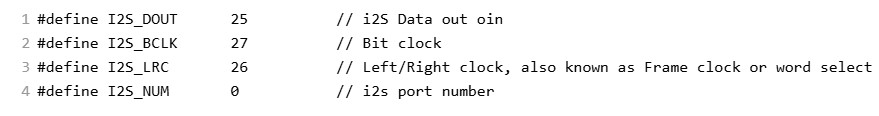
\includegraphics[width=0.7\linewidth]{Images/pins_i2s.jpeg}
    \caption{Declaració dels pins de la ESP32 assignats a cada senyal del bus I2S.}
    \label{pins_i2s_fig}
\end{figure}

\par Un cop declarades les variables de configuració esmentades, és necessari per inicialitzar el canal d'I2S correctament, fer ús de les següents funcions:
\begin{itemize}
    \item \textbf{\textit{i2s{\_}driver{\_}install}:} funció que instala el driver del protocol I2S a la ESP32 al port referenciat dins els arguments de la pròpia funció. A més, cal incluir en aquests arguments la variable \textit{i2s{\_}config} de configuració del canal.
    \item \textbf{\textit{i2s{\_}set{\_}pin}:} funció que assigna els pins del canal; utilitza la variable \textit{pin{\_}config} per configurar els ports amb els pins definits dins d'aquesta variable. 
\end{itemize}

\par Finalment, degut a que només es necessita enviar informació pel bus I2S, només serà necessari fer ús de la funció \textit{i2s{\_}write} que permet escriure la informació al buffer d'I2S. Entre els arguments de la funció està el port I2S de la targeta ESP32, la direcció dins la memòria on està emmagatzemada la informació a transmetre, el tamany en bytes de la mostra a enviar pel SD, una variable de control per saber els bytes que s'han enviat i per últim, els ticks d'espera del scheduler del RTOS implementat en la ESP32 per enviar la mostra pel buffer.\cite{I2SESP32code}

\subsection{Muntatge de la font d'àudio}
\par El muntatge final de la font d'àudio es pot observar a la figura \ref{fig_fontaudioI2S} amb els components mencionats en el primer apartat d'aquest capítol, interconnectats en una mateixa protoboard. El codi final amb el que s'ha programat la targeta ESP32 es pot trobar a l'Annex 1.
\begin{figure}[H]
    \centering
    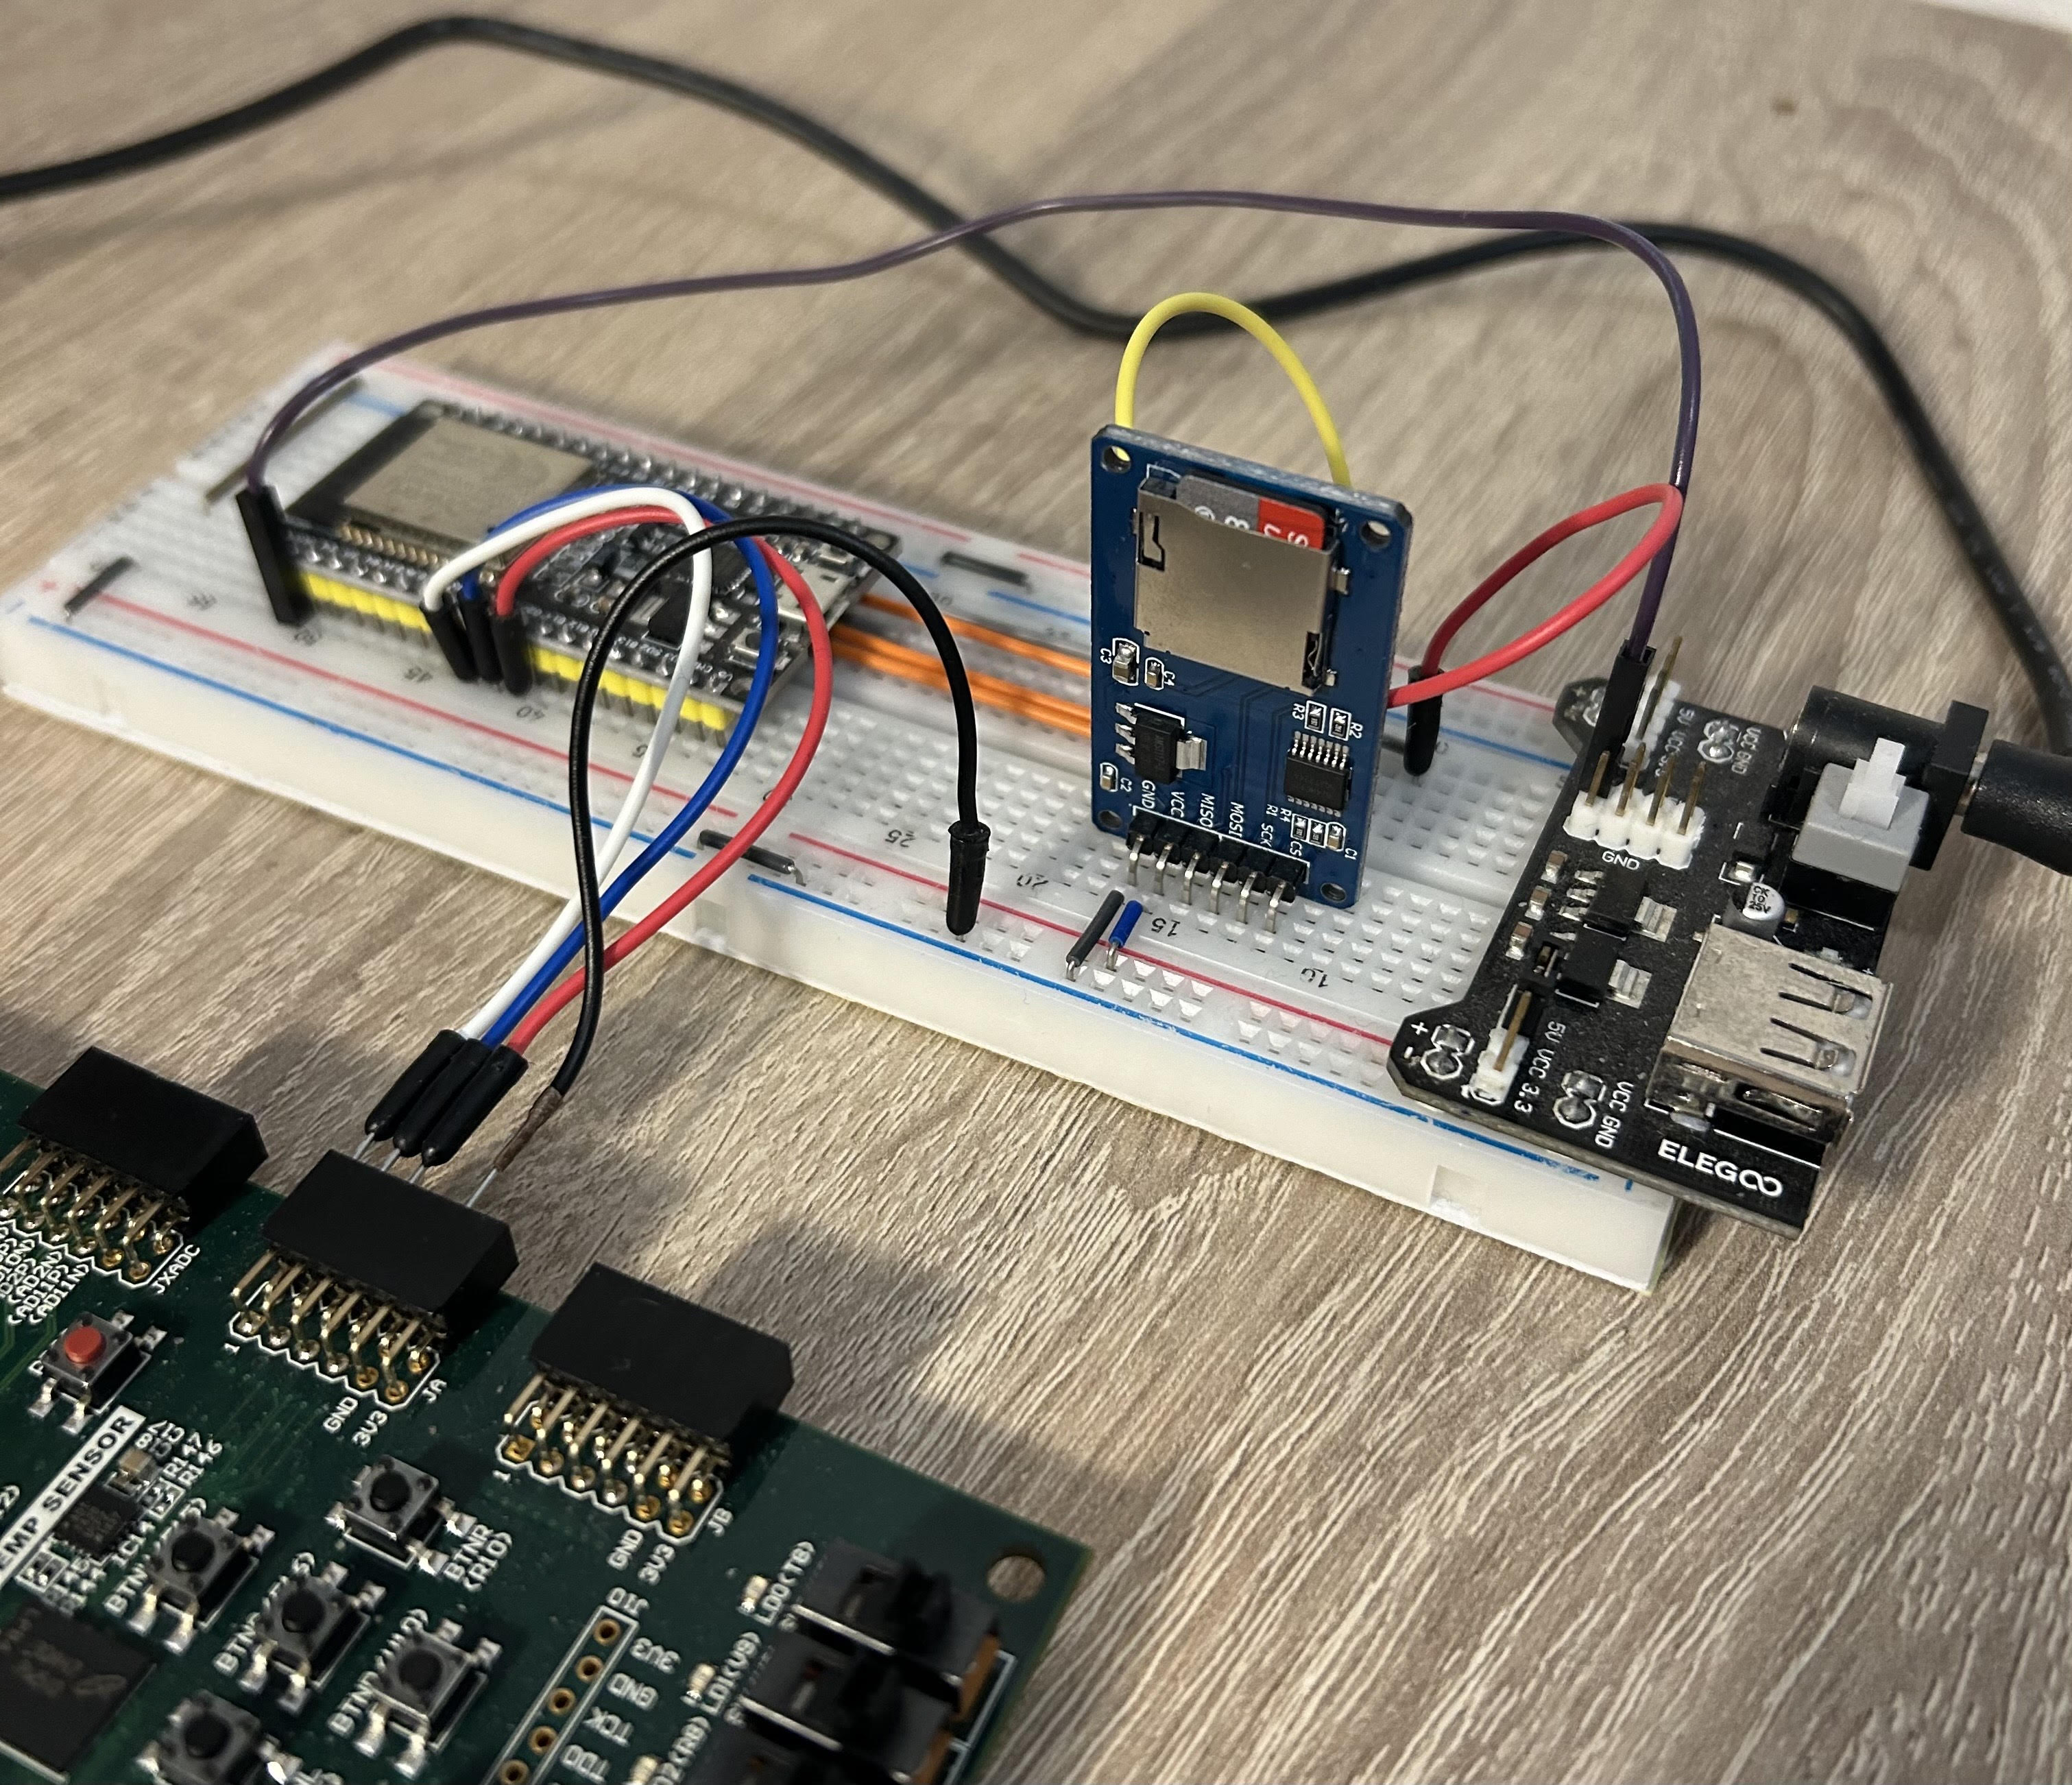
\includegraphics[width=0.4\linewidth]{Images/font_audio.jpg}
    \caption{Muntatge final de la font d'àudio I2S en una protoboard.}
    \label{fig_fontaudioI2S}
\end{figure}


 \section{Implementació del Receptor I2S}
 Per poder rebre correctament les mostres d'àudio transmeses pel bus I2S, s'ha dissenyat un receptor íntegrament en vhdl implementat a la FPGA. A continuació, es detalla el desenvolupament i execució del bloc.

 \subsection{Estructura de la entitat Receptora I2S}
 \par NXP (antigament Philips Semiconductors) ofereix possibles configuracions per la implementació del receptor I2S a \cite{I2S_manual}. A la figura \ref{receptor_i2s1_fig} es pot observar una d'aquestes configuracions. En aquest exemple, es pot apreciar que quan el senyal WS canvia de nivell, es genera un pols que provoca un reset del comptador de mòdul la longitud de la mostra d'àudio. Aquest comptador, genera polsos a les diferents senyals de sortida que activen els Flip Flops D i guarden el respectiu valor del bit. Quan WS canvia d'estat de nou, es transmet als registre de sortida del canal d'àudio que pertoqui, la mostra emmagatzemada en el conjunt de Flip Flops D i a continuació es resetejen. 

 \begin{figure}[H]
     \centering
     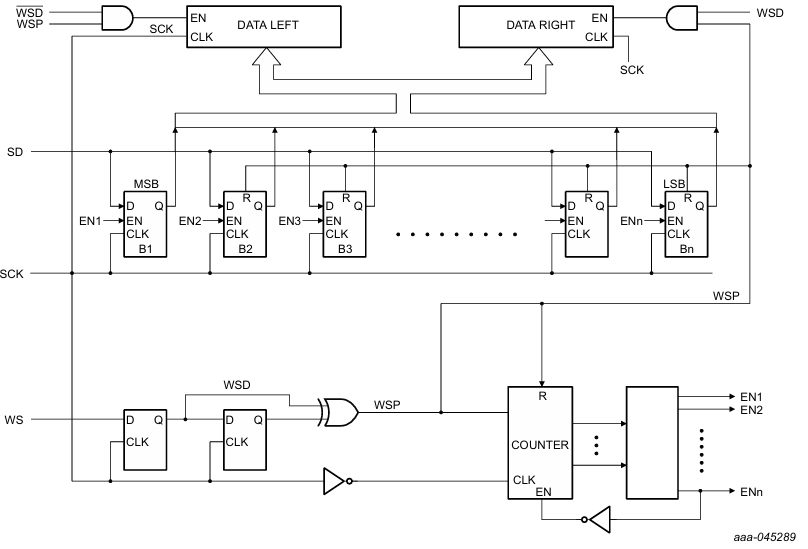
\includegraphics[width=0.6\linewidth]{Images/i2s_receiver_1.png}
     \caption{Una versió de la possible configuració del receptor I2S.\cite{I2S_manual}}
     \label{receptor_i2s1_fig}
 \end{figure}

 \par Una altra possible configuració que es mostren al manual \cite{I2S_manual} és la de la figura \ref{receptor_i2s2_fig}. En aquesta configuració, l'etapa de sortida és similar a la de la figura \ref{receptor_i2s1_fig}, essent composta de dos registres, un per canal d'àudio, i tants Flip Flops D com bits de la mostra samplejada. En aquesta implementació, el canvi d'estat del senyal WS també genera un pols que provoca un reset general dels Flip Flops de la sortida i del shift register que activa el Flip Flop D corresponent, segons el bit que s'està transmetent pel SD.
 \begin{figure}[H]
     \centering
     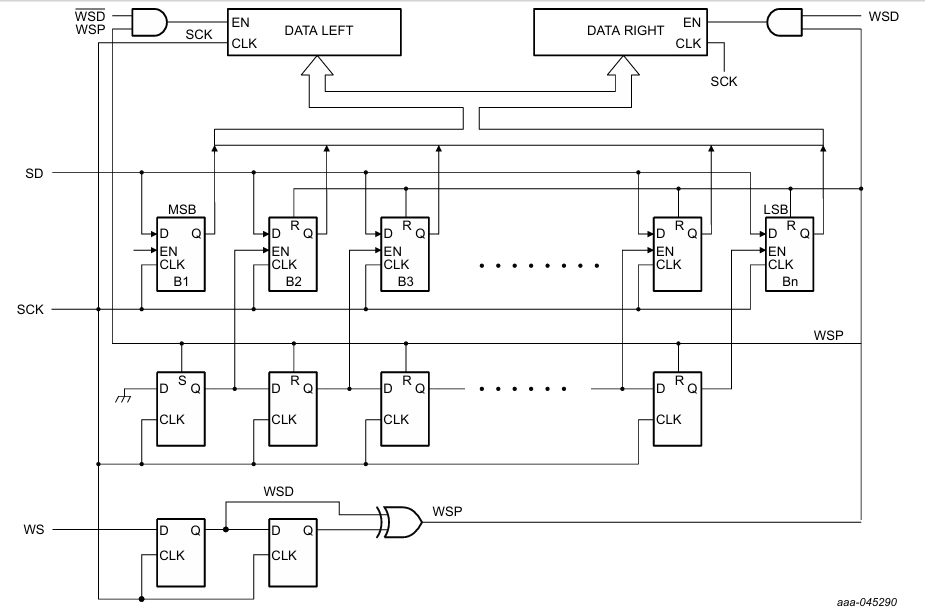
\includegraphics[width=0.6\linewidth]{Images/i2s_receiver_2.png}
     \caption{Una versió diferent de la figura \ref{receptor_i2s1_fig}, d'una possible configuració del receptor I2S. \cite{I2S_manual}}
     \label{receptor_i2s2_fig}
 \end{figure}

 \par Pel disseny del bloc receptor implementat a la FPGA s'han tingut en compte les configuracions comentades i finalment s'ha decidit per estructurar l'entitat com es pot veure a la figura \ref{diagrama_recI2S_fig}. El bloc receptor d'aquest treball implementa el comptador de bits de \ref{receptor_i2s1_fig} activat pel pols generat al canvi de nivell a WS. A diferència de les estructures exposades, la sortida es guarda en un registre SIPO. Un cop fet la lectura de la mostra transmesa pel bus I2S, es grava el valor en un registre PIPO.
 \begin{figure}[H]
     \centering
     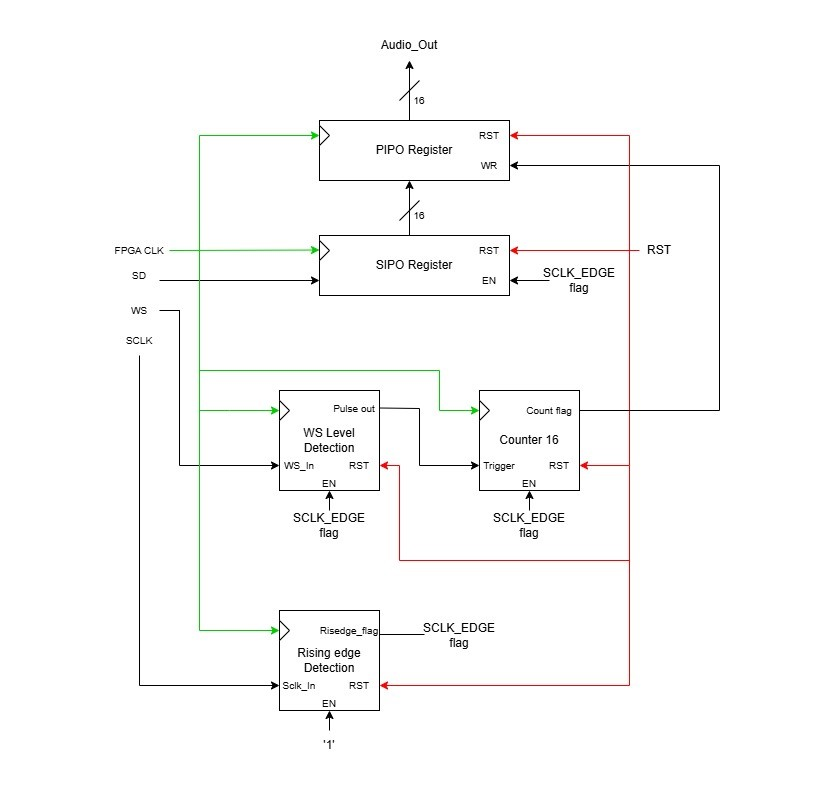
\includegraphics[width=0.55\linewidth]{Images/DiagramaTransceiverI2S.jpg}
     \caption{Diagrama de blocs de l'estructura implementada en el receptor I2S.}
     \label{diagrama_recI2S_fig}
 \end{figure}
 
 Els sub-blocs que el composen són els següents:
 \begin{itemize}
     \item \textbf{Rising Edge Detection:} Aquest bloc es un detector de flancs de pujada, que quan es detecta un canvi d'estat, de Low a High, es genera un pols al senyal de sortida. S'aplica a l'entrada el senyal SCLK per poder sincronitzar tots els blocs amb la flag de la sortida.
     \item \textbf{WS Level Detection:} El bloc genera un pols a la sortida quan el senyal d'entrada WS canvia d'estat. 
     \item \textbf{Counter 16:} Comptador de mòdul 16 que compta els flancs de pujada del SCLK. Quan arriba a 16, al port Count flag es genera un pols d'amplada un període del clk de la fpga, que activa la escriptura al registre PIPO de la sortida.
     \item \textbf{SIPO Register:} Registre SIPO per emmagatzemar el valor de la mostra d'àudio transmesa pel SD.
     \item \textbf{PIPO Register:} Registre PIPO on s'emmagatzema la mostra d'àudio a la sortida.
 \end{itemize}
 
\subsection{Banc de proves del receptor I2S}
\par Finalment, es procedeix a la validació de les funcionalitats del bloc receptor en conjunt. Degut a que l'entitat és de creació pròpia, és necessari testejar-lo amb un banc de proves. Per això, es simulen els senyals del bus I2S i el clock de la FPGA, tot mantenint els timings esperats. \par Com es pot apreciar a la figura \ref{figtestbenchI2S}, la mostra \textit{input\textunderscore 1} es captura a la sortida un cop s'han transmés els 16 bits de longitud del senyal. A continuació s'esmenen els requisits per al banc de proves:
\begin{itemize}
    \item \textbf{clock del sistema:} El període del clock del sistema és de 10 ns (100 MHz).
    \item \textbf{SCLK:} El període del serial clock del bus I2S esperat són 350 ns (2,85 MHz).
    \item \textbf{WS:} El període del WS esperat és de 32 cicles del rellotge sclk. 
    \item \textbf{SD:} Com ja s'ha explicat anteriorment, el mode d'operació del bus I2S és l'estàndard Philips, i en aquest mode, el MSB s'envia un període del sclk després del canvi al WS.
\end{itemize}
\begin{figure}[H]
    \centering
    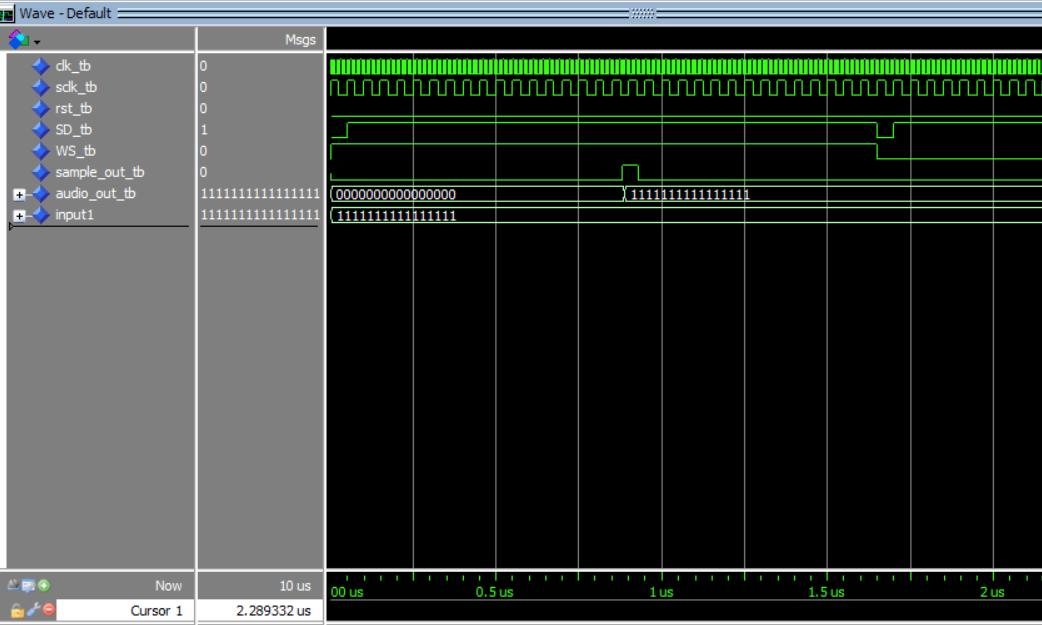
\includegraphics[width=0.6\linewidth]{Images/testbenchI2S.png}
    \caption{Cronograma del banc de proves pel receptor I2S.}
    \label{figtestbenchI2S}
\end{figure}

\section{Implementació a la FPGA}
\par Finalment, es sintetitza el codi VHDL del receptor al programa Vivado per evaluar els recursos consumits de la FPGA en la implementació del bloc. S'exposen els recursos de la FPGA utilitzats en la implementació del bloc a la taula \ref{taularecursosI2S}. Com es pot observar, el receptor I2S només utilitza blocs combinacionals per implementar les portes lògiques dels sub-blocs. En canvi, el major consum de recursos es deu als registres o blocs síncrons (FFs), que arriben a un total de 48.

\begin{table}[H]
    \centering
    \begin{tabular}{ | c | c | c | c | c | c |}
    \hline
    \centering
    \textbf{ID}     &  \textbf{LUTs} & \textbf{Registres}  & \textbf{Slices} & \textbf{Muxes}  & \textbf{DSPs} \\ [2ex] \hline
    \centering
    Receptor I2S    &  12 & 48  & 10 & 0  & 0 \\ \hline
    \end{tabular}
    \caption{Utilització de recursos de la FPGA pel bloc IP dissenyat.}
    \label{taularecursosI2S}
\end{table}

  